
\section{Superfluid Æther Framework}

We assume a stationary Euclidean 3-dimensional æther that behaves as a superfluid with zero viscosity and constant mass density. This continuous medium forms the basis of all physics: particles are topological vortex structures in the æther and fields correspond to flow patterns (vorticity, pressure, etc.). The dynamics are governed by classical flow equations, with the following fundamental postulates:

\begin{figure}[htbp]
    \centering
    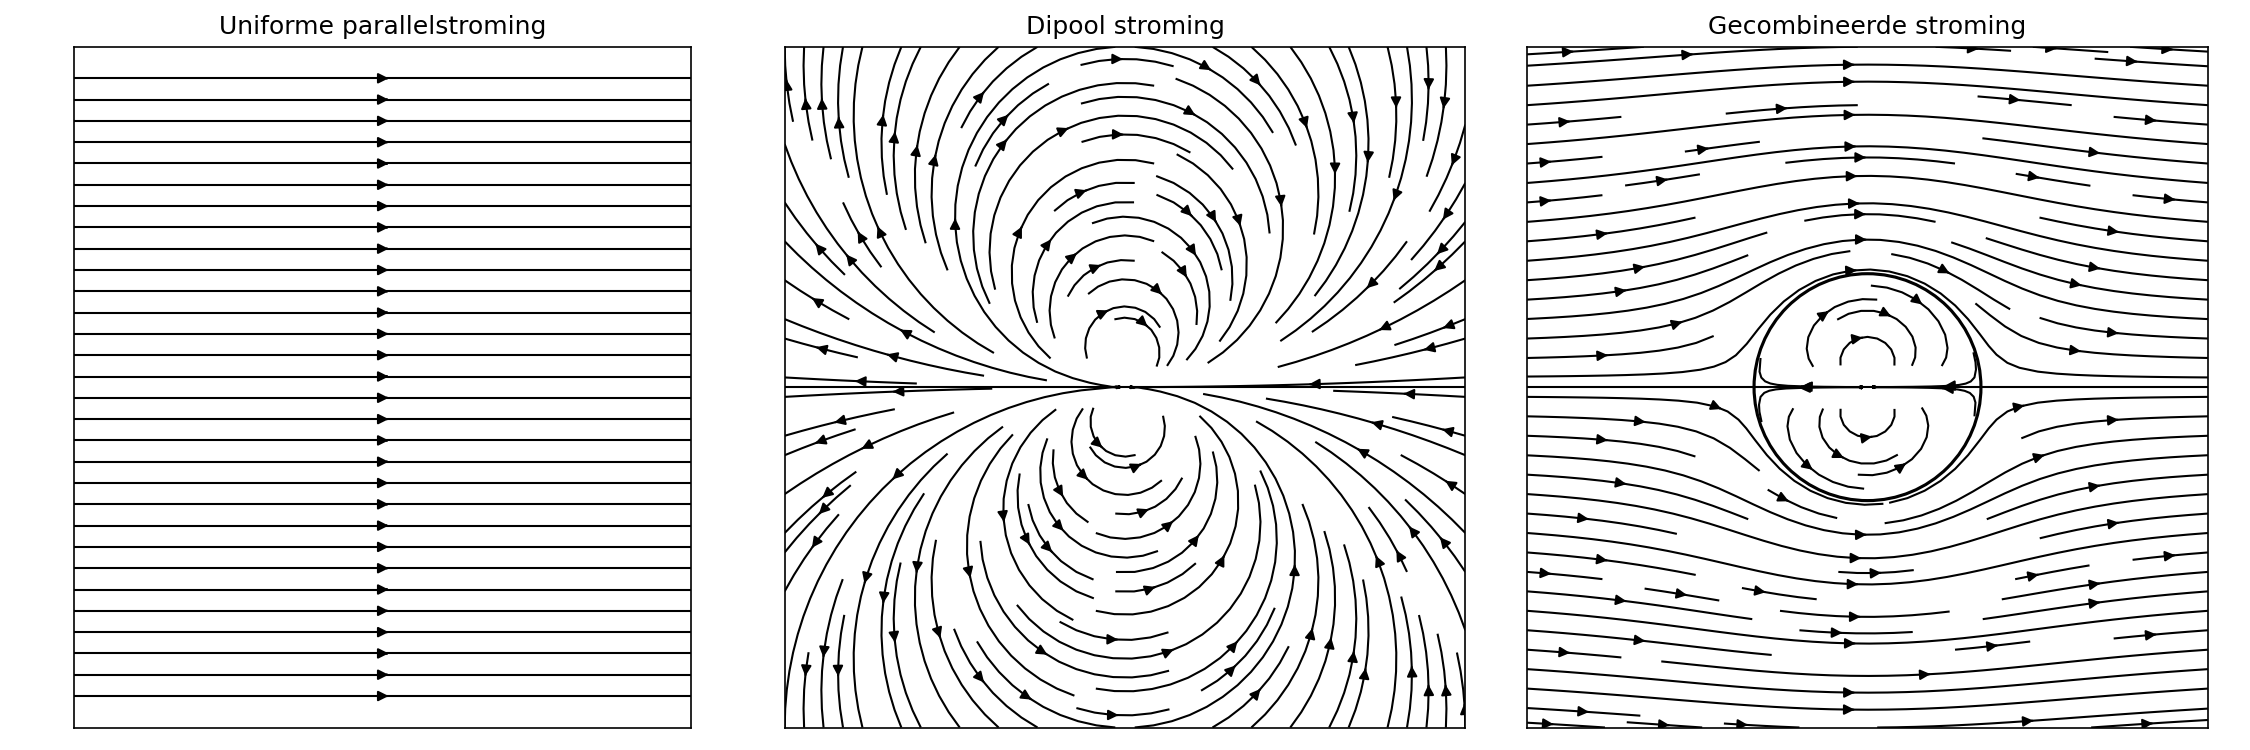
\includegraphics[width=0.85\textwidth]{03-combined_flow}
    \caption{Illustration of aether flow and vorticity around vortex cores.}
    \label{fig:vortexfields}
\end{figure}
\begin{description}
    \item[\textbf{Postulate I: Absolute flat space}] \hfill \\
    Space is a stationary, flat Euclidean background with a preferred frame defined by the æther at rest. All distances and velocities are measured in it. There is no intrinsic spacetime curvature; all metrics are derived from flow fields. (This is similar to Lorentz's original absolute frame concept, but now with a physical superfluid filling space~\cite{Winterberg2002-PlanckAether}).

    \item[\textbf{Postulate II: Incompressible uniform æther}] \hfill \\
    The æther is an ideal fluid with constant density $\rho_{\ae}$, zero viscosity, and zero compressibility (analogous to superfluid helium at $T=0$). Therefore, æther volume elements cannot be created or destroyed; Flow is divergenceless, except possibly at singular vortex cores. All local variations (e.g. near masses) are due to velocity fields or pressure, not to density changes.

    \item[\textbf{Postulate III: Vortex nodes as matter}] \hfill \\
    Matter particles are modeled as stable, topologically conserved vortex nodes. According to Kelvin~\cite{Kelvin1867-vortex}, an atom or fundamental particle is a quantized vortex loop or node in the æther. It has a well-defined core (of the order of the Planck length $l_{\textrm P}$ in radius, according to the Planck-æther theories~\cite{Winterberg2002-PlanckAether}) around which æther flows circularly. The topology of the vortex (node type) might correspond to the type of particle, while the intrinsic angular velocity $\omega$ (the vortex velocity of æther around the nucleus) gives the particle its internal clock.

    \item[\textbf{Postulate IV: Time as nucleus rotation}] \hfill \\
    The proper time for a particle is defined by the rotation of its vortex core. For example, a certain fixed rotation angle (say one full $2\pi$ revolution of the core) might define a fixed amount of proper time (perhaps on the order of one \("\)tick\("\)). The age or internal time of a particle advances with the number of revolutions its core performs. Faster nucleus rotation means a faster internal time rate. Importantly, this rotation is an absolute physical process that occurs relative to the æther.

    \item[\textbf{Postulate V: Thermodynamics as emergent behavior}] \hfill \\
    Temperature, entropy, and thermal fluctuations arise statistically from microscopic æther flow. Fundamentally, however, the medium is nonthermal and perfectly dissipationless. In most of the æther (far from vortex cores), the flow can be irrotational and laminar. Macroscopic thermodynamic concepts (temperature, entropy) are assumed statistically to arise from small-scale æther dynamics, but at the fundamental level, the æther is a dissipationless, nonthermal medium. Therefore, we ignore any finite-temperature or viscous effects – the æther is a perfectly inviscid fluid. Only vortex interactions and pressure fields play a role.

    \item[\textbf{Postulate VI: Forces via vorticity}] \hfill \\
    All forces (electromagnetism, gravity, etc.) are mediated by æther flows.
    Spatial gradients in vorticity or helicity (twisting of vortex lines) in the æther field can influence other vortices. For example, what we observe as a $\text{"gravitational field"}$ will be modeled by a certain æther velocity field (as we will explain later). The principle of maximum force $ F_\text{max} = c^4 / 4 G $ from general relativity~\cite{Schiller2022-maxforce}, which sets an upper limit on force in nature, is assumed to arise from properties of the æther (e.g., maximum flow velocity $c$ and density $\rho_\text{\ae}$ impose a limit on momentum flux/force).
\end{description}

Within this framework, the æther provides an absolute reference for motion, but any measurable effects must ultimately be consistent with relativity. As Winterberg (2002) put it, ``the universe can be regarded as Euclidean flat spacetime, provided we include a densely populated quantum vacuum superfluid as æther''~\cite{Winterberg2002-PlanckAether}.

\begin{figure}[htbp]
    \centering
    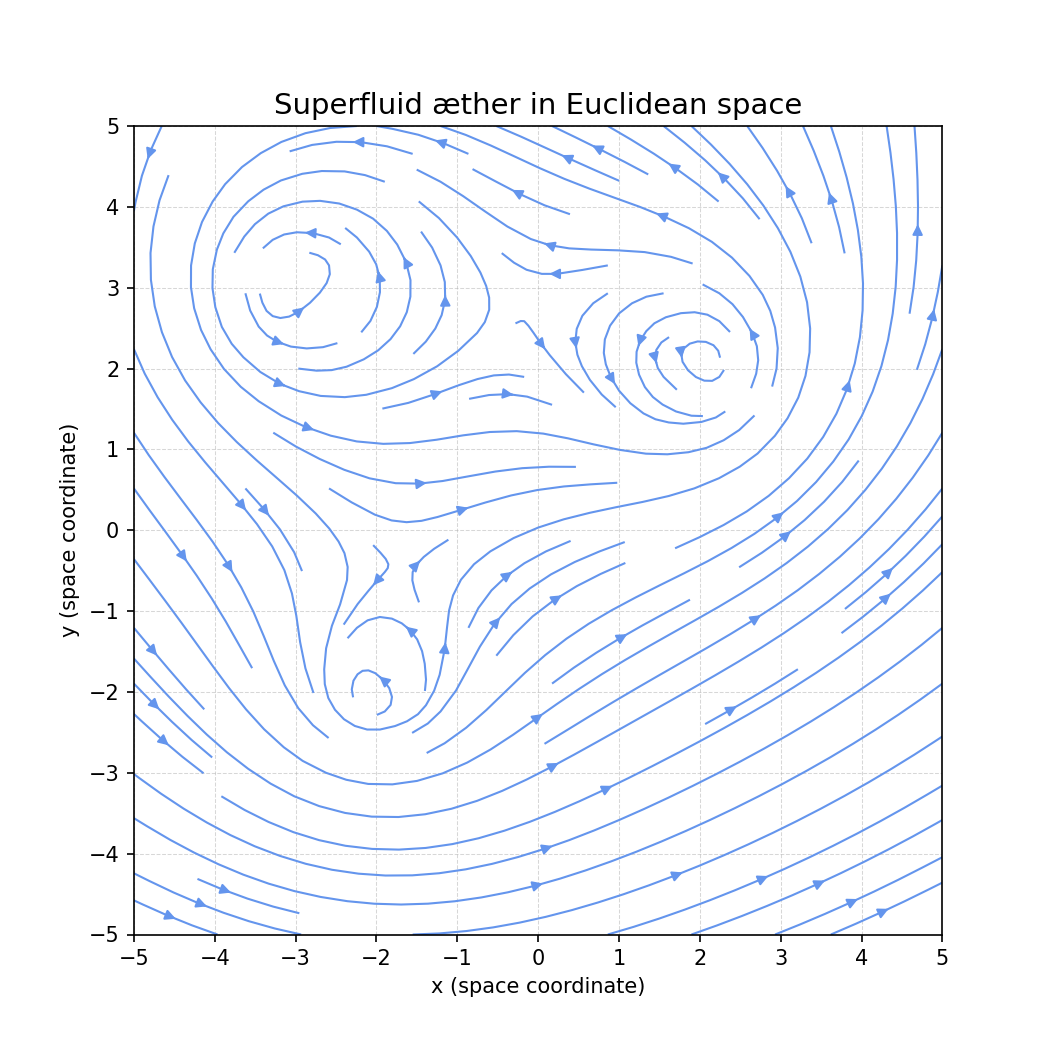
\includegraphics[width=0.85\textwidth]{04-ÆtherSuperfluïde}
    \caption{Uniform æther flow with embedded vortex structures. The æther is proposed as an ideal superfluid with conservation of vorticity.}
    \label{fig:ÆtherSuperfluïde}
\end{figure}


\textbf{Definitions and Constants:} For later use, we define some fundamental constants in this model. The Planck time is
\[
    t_{\textrm P} = \sqrt{\frac{\hbar G}{c^5}} \approx 5.39\times10^{-44}\ \text{s},
\]
the natural unit of time in quantum gravity. It represents approximately the time taken by light to travel one Planck length $l_{\textrm P} \approx 1.62\times10^{-35}$ m. In many superfluid æther theories, $l_{\textrm P}$ could be the core diameter of elementary vortex structures~\cite{Winterberg2002-PlanckAether}, so one complete rotation of an elementary vortex structure with the speed of light $c$ would take the order of $t_{\textrm P}$. Thus, $t_{\textrm P}$ sets an upper bound on the rotation frequency ($\sim 10^{43}$ s$^{-1}$) for any physical clock in the æther.

Another useful constant is the proposed maximum force:
\begin{equation*}
    F_\text{max} = \frac{c^4}{4G} \approx 3.0\times10^{43}\ \text{N}.
\end{equation*}

This appears as an upper limit in general relativity~\cite{Schiller2022-maxforce}, for example, the gravitational attraction between two black holes cannot exceed $F_{\textrm max}$. In the æther picture, $F_{\textrm max}$ can be interpreted as the maximum stress or drag force the superfluid æther can sustain when flows approach the speed of light.

We retain $c$ (speed of light in vacuum) as the characteristic signal speed in the æther (e.g., the speed of sound or wave propagation in the superfluid vacuum, often taken as $c = \sqrt{B/\rho_{\text{\ae}}}$ for bulk modulus $B$). The Newtonian gravitational constant $G$ will enter when linking æther flow to mass (since mass is essentially a vortex with a certain circulation and core structure that relates to $G$). We will introduce any additional constants as needed.